% ═══════════════════════════════════════════════════════════════════════
\section{Une application : la méthode de Newton-Raphson}
% ═══════════════════════════════════════════════════════════════════════

\begin{frame}{Un zéro, vu comme un point fixe}
  \small Soit $f:\R\to\R$ deux fois dérivable, et $x^\star$ un zéro de
  $f$ avec $f'(x^\star)\neq0$. Plutôt que de résoudre $f(x)=0$, on pose
  \[
    g(x) = x - \frac{f(x)}{f'(x)}\qquad(\text{là où } f'(x)\neq0).
  \]
  Puisque $f(x^\star)=0$ : $g(x^\star)=x^\star$.
  \vspace{4pt}
  \begin{center}
    Un zéro de $f$ est un point fixe de $g$.\\[2pt]
    La méthode consiste à itérer $g$ : $x_{n+1}=g(x_n)$.
  \end{center}
\end{frame}

\begin{frame}{Proposition 2.9 --- $g$ est localement une contraction}
  \begin{Enonce}{Proposition 2.9}
    \small Avec les notations précédentes, $g'(x^\star)=0$. Par
    conséquent, pour tout $k\in\intoo{0}{1}$, il existe $\delta>0$ tel que
    $g$ soit une contraction de rapport $k$ sur l'intervalle fermé
    $I=[x^\star-\delta,\,x^\star+\delta]$.
  \end{Enonce}
  \begin{AuTableau}
    \footnotesize Calcul : $g'(x) = f(x)f''(x)/f'(x)^2$, nul en $x^\star$.
    Par continuité, $|g'|\leq k$ près de $x^\star$ (réduire $\delta$
    pour avoir aussi $g(I)\subseteq I$) ; puis théorème des
    accroissements finis.
  \end{AuTableau}
  \begin{Rem}{Remarque 2.12 --- Complétude de l'intervalle}
    \footnotesize $I\subset\R$, pas $\R^2$ : on utilise la forme
    générale (remarque 2.11). Fait admis : un sous-ensemble
    fermé d'un espace complet est complet. $I$ est fermé dans
    $\R$, complet : Banach s'applique.
  \end{Rem}
\end{frame}

\begin{frame}{Figure 2.17 --- Interprétation géométrique}
  \begin{columns}[c]
    \begin{column}{0.44\textwidth}
      \small $f(x)=(x-2)^2-3$, $x_0=5$.
      \begin{itemize}
        \item Tangente en $(x_0,f(x_0))$ jusqu'à l'axe des $x$ :
          $x_1=4$.
        \item On recommence : $x_2=\num{3.75}$.
        \item À comparer : $x^\star=2+\sqrt3\approx\num{3.732}$.
      \end{itemize}
      \vspace{4pt}
      Banach garantit la convergence pour tout $x_0\in I$.
    \end{column}
    \begin{column}{0.54\textwidth}
      \FigBox[0.62\textheight]{%
        \begin{tikzpicture}[xscale=1.3, yscale=0.5]
          \draw[axe] (1.6,0) -- (5.7,0) node[below, etiq]{$x$};
          \draw[sectioncolor, thick, domain=1.8:5.4, samples=60, smooth]
            plot (\x, {(\x-2)*(\x-2)-3}) node[right, etiq, sectioncolor]{$y=f(x)$};
          \draw[firebrick3, thick, domain=3.7:5.6] plot (\x, {6*\x-24});
          \draw[coveraccent, thick, domain=3.4:4.7] plot (\x, {4*\x-15});
          \draw[sectioncolor!40, thin, dotted] (5,0) -- (5,6);
          \draw[sectioncolor!40, thin, dotted] (4,0) -- (4,1);
          \node[pt, label={[etiq]above:$x_0$}] at (5,0) {};
          \node[pt, label={[etiq]above:$x_1$}] at (4,0) {};
          \node[ptim, label={[etiq]below:$x_2\approx x^\star$}] at (3.75,0) {};
        \end{tikzpicture}}
    \end{column}
  \end{columns}
\end{frame}

\begin{frame}{Convergence quadratique}
  \small Banach seul garantit une convergence géométrique :
  l'erreur est multipliée par au plus $k$ à chaque étape.
  \vspace{6pt}

  Mais ici $g'(x^\star)=0$ exactement (et pas seulement
  $|g'(x^\star)|\leq k$). Un développement de Taylor plus fin montre que
  la convergence est quadratique :
  \begin{center}
    le nombre de décimales exactes double à peu près à chaque
    itération,
  \end{center}
  une fois assez près de $x^\star$.
\end{frame}

\begin{frame}{Exemple 2.11 --- Deux méthodes, une même équation}
  \small Équation $\cos(x)=x$, solution $x^\star\approx\num{0.7390851332}$.
  \begin{itemize}
    \item Méthode simple $x_{n+1}=\cos(x_n)$, depuis $x_0=0$ :
      converge (contraction de rapport $\sin(1)\approx\num{0.841}$), mais
      il faut $21$ itérations pour $4$ décimales et $45$ pour $8$.
    \item Newton sur $f(x)=\cos(x)-x$ :
      $g(x) = x+\dfrac{\cos(x)-x}{\sin(x)+1}$, depuis $x_0=1$.
  \end{itemize}
  \begin{center}
  \begin{tabular}{ccc}
    \toprule
    $n$ & $x_n$ & erreur $|x_n-x^\star|$ \\
    \midrule
    $0$ & $\num{1.000000000}$ & $\num{2.6e-1}$ \\
    $1$ & $\num{0.750363868}$ & $\num{1.1e-2}$ \\
    $2$ & $\num{0.739112891}$ & $\num{2.8e-5}$ \\
    $3$ & $\num{0.739085133}$ & $\num{1.9e-10}$ \\
    \bottomrule
  \end{tabular}
  \end{center}
  \small Trois itérations de Newton battent les $45$ de la méthode simple :
  $1$ ; $2$ ; $5$ ; $10$ ; … décimales exactes.
\end{frame}

\begin{frame}{Exemple 2.12 --- Une boîte à coût minimal (1/2)}
  \small Boîte sans couvercle, base carrée de côté $x$, volume
  $V=800$~cm$^3$, donc hauteur $h=800/x^2$.
  \begin{itemize}
    \item base : $\num{0.05}$~\$/cm$^2$ ; parois : $\num{0.02}$~\$/cm$^2$ ;
    \item bordure de renfort sur le pourtour de l'ouverture (périmètre
      $4x$) : $\num{0.08}$~\$/cm.
  \end{itemize}
  \[
    C(x) = \underbrace{\num{0.05}\,x^2}_{\text{base}}
    + \underbrace{\num{0.02}\cdot4xh}_{\text{parois}}
    + \underbrace{\num{0.08}\cdot4x}_{\text{bordure}}
    = \num{0.05}\,x^2 + \frac{64}{x} + \num{0.32}\,x.
  \]
  Minimiser : résoudre
  $f(x)\coloneqq C'(x) = \num{0.10}\,x - \dfrac{64}{x^2} + \num{0.32} = 0$,
  soit la cubique $\num{0.10}\,x^3+\num{0.32}\,x^2-64=0$ --- aucune racine
  évidente.
\end{frame}

\begin{frame}{Exemple 2.12 --- Une boîte à coût minimal (2/2)}
  \small Newton sur $f$, avec $f'(x)=\num{0.10}+128/x^3$, depuis $x_0=8$
  (une boîte presque cubique) :
  \begin{center}
  \begin{tabular}{ccc}
    \toprule
    $n$ & $x_n$ (cm) & $f(x_n)$ \\
    \midrule
    $0$ & $\num{8.000000}$ & $\num{0.1200}$ \\
    $1$ & $\num{7.657143}$ & $\num{-5.84e-3}$ \\
    $2$ & $\num{7.672315}$ & $\num{-1.28e-5}$ \\
    $3$ & $\num{7.672348}$ & $\num{-6.20e-11}$ \\
    \bottomrule
  \end{tabular}
  \end{center}
  \vspace{4pt}
  Côté de base $x^\star\approx\num{7.672}$~cm, hauteur
  $h^\star=800/(x^\star)^2\approx\num{13.59}$~cm, coût total
  $\approx\num{13.74}$~\$.
  \vspace{4pt}

  Trois itérations suffisent largement pour fabriquer une boîte.
\end{frame}

\begin{frame}{Note historique 2.3 --- Stefan Banach (1892--1945)}
  \footnotesize
  \begin{columns}[T]
    \begin{column}{0.25\textwidth}
      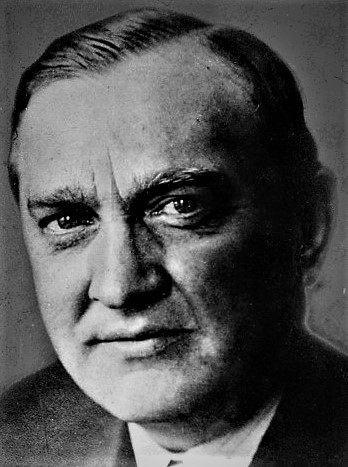
\includegraphics[width=\linewidth]{stefan-banach.jpg}\\
      {\scriptsize\color{gray}Stefan Banach (1892--1945).
      Domaine public, Wikimedia Commons.}
    \end{column}
    \begin{column}{0.72\textwidth}
      \begin{itemize}
        \item Né à Cracovie, confié à des familles d'accueil ; apprend
          une grande partie des mathématiques par lui-même.
        \item 1916 : Hugo Steinhaus surprend, dans un parc, une
          conversation de Banach sur l'intégrale de Lebesgue. Il lui
          propose des problèmes ouverts ; Banach les résout en une
          semaine. « Ma plus grande découverte scientifique a été de
          découvrir Banach. »
        \item Thèse (1920, publiée en 1922) : définit les espaces
          de Banach et fonde l'analyse fonctionnelle moderne --- le
          théorème du point fixe y apparaît.
      \end{itemize}
    \end{column}
  \end{columns}
\end{frame}

\begin{frame}{Note historique 2.3 (suite)}
  \small
  \begin{itemize}
    \item Professeur à Lwów (aujourd'hui Lviv, Ukraine), il y fonde avec
      ses collègues l'école mathématique de Lwów.
    \item On se réunit au Café Écossais ; les problèmes ouverts
      sont consignés dans un cahier resté célèbre : le Livre
      écossais.
    \item Sous l'occupation allemande, il échappe à la déportation en
      travaillant comme « nourricier de poux » dans un institut de
      recherche sur le typhus --- emploi qui protégeait alors de
      nombreux universitaires.
    \item Il meurt d'un cancer du poumon en 1945, peu après la fin de la
      guerre, à $53$ ans.
  \end{itemize}
\end{frame}

\begin{frame}{Note historique 2.4 --- Origines et applications du théorème}
  \small
  \begin{itemize}
    \item Picard (1890) utilise déjà les approximations
      successives pour l'existence et l'unicité des solutions de
      certaines équations différentielles (théorème de
      Picard-Lindelöf).
    \item Banach (1922) : le cadre abstrait. En isolant
      la complétude et le caractère contractant, un seul résultat
      couvre de nombreux problèmes.
    \item Caccioppoli (1930) le redécouvre indépendamment :
      théorème de Banach-Caccioppoli.
  \end{itemize}
  \vspace{4pt}
  Applications : construction des fractales (chapitre 3) ;
  Newton et autres méthodes numériques ; PageRank, qui a classé
  les pages web chez Google à ses débuts --- le point fixe d'une
  contraction dans un espace de dimension égale au nombre de pages du
  Web (chapitre 4).
\end{frame}
